\documentclass[11pt]{article}
\usepackage[T1]{fontenc}
\usepackage[utf8]{inputenc}
\usepackage{lmodern,microtype,amsmath,amssymb,amsthm,mathtools}
\usepackage[margin=28mm]{geometry}
\usepackage{booktabs,array,enumitem,tikz}
\usetikzlibrary{arrows.meta,calc,positioning}
\usepackage[unicode,colorlinks=true,linkcolor=blue!45!black,
 citecolor=green!35!black,urlcolor=blue!55!black]{hyperref}
\usepackage{xurl}
\setlength{\emergencystretch}{3em}
\numberwithin{equation}{section}
\newtheorem{theorem}{Theorem}[section]
\newtheorem{lemma}[theorem]{Lemma}
\newtheorem{proposition}[theorem]{Proposition}
\newtheorem{corollary}[theorem]{Corollary}
\theoremstyle{definition}
\newtheorem{definition}[theorem]{Definition}
\newtheorem{remark}[theorem]{Remark}
\newcommand{\ii}{\mathrm i}
\newcommand{\Vol}{\operatorname{Vol}}
\newcommand{\Cen}{\mathrm C}
\newcommand{\Lft}{\mathrm L}
\newcommand{\Rgt}{\mathrm R}
\newcommand{\calQ}{\mathcal Q}
\newcommand{\Rea}{\operatorname{Re}}
\title{Balanced circle packings from terminal tangle decorations}
\author{}
\date{2 November 2026}
\begin{document}
\maketitle

\begin{abstract}
A matched triangulation of the sphere specifies an augmented link and
a complete circle packing. We give a finite modification near its
crossing disks that makes a strict shared-face inequality hold at
every crossing region. The modification leaves every original circle
fixed and inserts an even number of terminal tangles on each side of
each original region. The two insertion counts are chosen by an
explicit formula. Their geometric recurrence and an integral for the
normalized triangle action prove strict balance for every retained
and added region, including regions adjacent to the two marked lines.
Odd powers in the added tangles preserve the original endpoint
pairing. The shared-face criterion then gives the volume limit for
the resulting fixed knots after independently sufficiently long
signed fillings. The construction can change the knot; all powers
and all decorations are fixed before the level tends to infinity.
\end{abstract}

\section{The diagram, the inequality, and the result}

A \emph{marked matched sphere} consists of a finite oriented simple
triangulation of the two-sphere, a perfect matching of its dual
graph, and a chosen edge outside that matching. A dual matching edge
pairs two adjacent triangles. We also call their common primal edge
a matching edge. Every triangle belongs to exactly one pair.
The chosen nonmatching edge is the \emph{mark}.
Simplicity means that edges have distinct endpoints, no two vertices
are joined by more than one edge, and every face is a triangle with
three distinct vertices. There are at least four vertices.

The inverse projection and crossing-disk cut places a two-strand
crossing-circle region at each matched pair and joins its four
terminals along the remaining dual edges. It gives an augmented
link in \(S^3\). A crossing circle bounds the specified disk meeting
the main strands twice. The cyclic order and the frame of that disk
are part of the data. We retain either no crossing or a signed half
twist \(\epsilon_e\in\{-1,0,1\}\) at each region \(e\).
Filling the crossing circle along its disk-framed primitive slope
\(\mu_e+p_e\lambda_e\) produces the physical power
\begin{equation}\label{td:powers}
 n_e=\epsilon_e-2p_e .
\end{equation}
Its parity is fixed by \(\epsilon_e\). We require that the chosen
parities join the main strands into one knot, with no additional
closed main component.

The complete packing can be normalized by sending the contact at
the mark to infinity. Its two incident white circles become
parallel lines. Their curvatures are zero; every other white circle
has positive curvature \(w_f\), the reciprocal of its Euclidean
radius. We call these remaining vertices ordinary. All occurrences
of a vertex refer to the same circle and the same weight.

The action used below has a fixed additive normalization. Define
\[
 \Lambda(t)=-\int_0^t\log(2\sin s)\,ds,\qquad
 e(a)=\frac{\Lambda(\pi a)+\Lambda(\pi/2-\pi a)}{\pi},
 \quad 0\le a\le\tfrac12 ,
\]
and, for nonnegative weights with at least one positive entry, put
\begin{equation}\label{td:entropy}
 \calQ(w_1,w_2,w_3)=
 \max_{\substack{a_i\ge0\\\sum_i a_i=1/2\\a_i=0\ {\rm if}\ w_i=0}}
       \left\{\sum_i e(a_i)+\sum_{w_i>0}a_i\log w_i\right\}.
\end{equation}
In particular \(\calQ(0,w,0)=\frac12\log w\).
This is the triangle action in the shared-face coefficient estimate;
we do not add a constant depending on the triangle.

At a matched pair the two oriented triangles are
\((x,b,y)\) and \((y,c,x)\). Its cyclic boundary tuple is
\((x,b,y,c)\). We write
\begin{equation}\label{td:ordering}
 H(x,b,c,y)
\end{equation}
for a local source polynomial: its outer variables are \(x,y\),
and its input and output middle variables are \(b,c\).
Thus the argument order in \eqref{td:ordering} differs from the
cyclic boundary order. The same letters will denote the corresponding
curvatures when no polynomial is being evaluated.
The matching edge \(xy\) cannot be the marked nonmatching edge, so
\begin{equation}\label{td:outer}
 A=x+y>0,\qquad P=xy,\qquad \rho=P/A^2\in[0,1/4].
\end{equation}

\begin{definition}[Strict complete balance]\label{td:balance}
A region with weights \((x,b,c,y)\) is strictly balanced if
\[
 X:=\calQ(x,b,y)+\calQ(x,c,y)>\log b\quad(b>0),\qquad
 X>\log c\quad(c>0).
\]
A comparison with a zero middle is omitted.
\end{definition}

\begin{theorem}[Finite balanced decoration]\label{td:main}
Fix a marked matched sphere with its crossing-disk frames and a
knot parity pattern. There is a finite decoration by terminal
crossing-circle tangles with the following properties.
\begin{enumerate}[label=\textup{(\roman*)},leftmargin=*]
\item At each original region an even nonnegative number of
terminals is inserted on each of its two shaded sides. No original
crossing circle is removed.
\item The refined white sphere is simple and has its original
nonmatching marked edge. Its complete packing extends the original
packing, leaving every old circle fixed.
\item Every original and added crossing region is strictly balanced
at this one complete packing.
\item Give every added terminal an odd power, of either sign.
The four-endpoint pairing at each decorated original region is
unchanged, and no internal main component is created.
\end{enumerate}
The insertion counts are the explicit integers in
\eqref{td:counts}. The construction uses no bound on the number
of regions and no acyclicity assumption on the original diagram.
\end{theorem}

\begin{corollary}[Filled knot volume]\label{td:volume}
Let \(\widehat D\) be a fixed decorated diagram from
Theorem~\ref{td:main}. Retain the original knot parity pattern and
odd parity at every added terminal. There is a threshold
\(T_{\widehat D}\) such that, for every fixed collection of integers
\(p_e\) with \(|p_e|\ge T_{\widehat D}\), independently in sign and
size, the resulting knot \(K_{\boldsymbol p}\) is hyperbolic and
\begin{equation}\label{td:volume-limit}
 \lim_{N\to\infty}\frac{2\pi}{N}
      \log\left|\langle K_{\boldsymbol p}\rangle_N\right|
       =\Vol(S^3\setminus K_{\boldsymbol p}).
\end{equation}
Here \(\langle K\rangle_N\) is the reduced zero-framed Kashaev
invariant, with unknot value one and parameters
\(q_N=e^{\pi\ii/N}\), \(q_N^2=e^{2\pi\ii/N}\). The limit runs
through both parities and composite levels.
\end{corollary}

The original regions, as well as the added ones, must be filled
sufficiently long. Their signed powers and the decoration are fixed
before \(N\). There is no asserted uniform filling threshold over
different diagrams or a simultaneous growing-diagram limit.
Preserving an endpoint pairing does not preserve the isotopy type
of the filled knot.

Circle patterns and ideal-polyhedral descriptions of fully augmented
links are classical; see Purcell~\cite{Purcell}. Gluing along the
associated thrice-punctured spheres belongs to the setting of
belted sums, studied for fully augmented links by
Morgan--Ransom--Spyropoulos--Trapp--Ziegler~\cite{Belted}.
Volume-conjecture results for Whitehead chains and augmented knotted
trivalent graphs appear in van der Veen~\cite{Whitehead,Trivalent}.
We do not claim that the knot families here are disjoint from those
classes. The result proved here is the finite, even terminal
construction enforcing the specified normalized inequality on
an arbitrary fixed marked simple sphere.

\section{The imported geometry and coefficient criterion}

We state precisely what is used from the companion papers. This
allows the local construction below to be read without importing
another full asymptotic argument.

\begin{proposition}[Companion interface]\label{td:imports}
For a fixed marked matched sphere:
\begin{enumerate}[label=\textup{(\roman*)},leftmargin=*]
\item Proposition 2.1 and Section 2 of \cite{Marked} construct the
packing, its supporting right-angled polyhedra and the original
augmented exterior with labeled disk curves. The complete
potential is
\[
 P_D(q)=\sum_{\text{triangles }t}\calQ((e^{q_f})_{f\in t})
                    -\sum_{f\ {\rm ordinary}}q_f .
\]
Its minimum is
\(\Phi_D=\Vol(Y_D)/(2\pi)\), where \(Y_D\) is that exterior;
the two protected entries are kept exactly zero.
\item Proposition 4.1, Theorem 9.1 and Corollary 9.2 of
\cite{Finite} identify the actual marked spectral source at
level \(N\ge3\), with \(d=N-1\), as
\begin{equation}\label{td:source}
 S_{D,N}(\boldsymbol\sigma)=
 \left[\prod_{f\ {\rm ordinary}} L_f^d\right]
 \left.\prod_e H_{V_N}(L_{x_e},L_{b_e},L_{c_e},L_{y_e};\sigma_e)
                                      \right|_{L_u=L_v=0}.
\end{equation}
Here \(u,v\) are the endpoints of the mark, and
\[
 V_N(\sigma;z)=
 \frac{\chi_N(\sigma)-\chi_N(z)}{\sigma-z},\qquad
 \chi_N(z)=2T_N(z/2)+2
\]
is a polynomial divided difference. The local Casimir is substituted
for \(z\); \(T_N(\cos\phi)=\cos(N\phi)\).
The homogeneous polynomial has degree \(d\) in the face variables
and degree at most \(d\) in \(\sigma\). The theorem retains cups,
caps, the original mark, even-level grids and repeated-root normals.
\item Theorem 1.1 of \cite{Local} gives the three local upper rates
\begin{equation}\label{td:rates}
 \begin{aligned}
 A_{\Cen}&=X,\\
 A_{\Lft}&=\max\{\log c,\calQ(x,b,y)+\tfrac12\log c\},\\
 A_{\Rgt}&=\max\{\log b,\calQ(x,c,y)+\tfrac12\log b\}.
 \end{aligned}
\end{equation}
The estimates are uniform for all face phases and
\(\sigma\in[-2,2]\), with fixed positive ordinary moduli and exact
protected zeros. An overloaded zero middle removes that one-sided
sector. Their hypothesis \(x+y>0\) is \eqref{td:outer}.
\item Definition 3.1 and Theorems 1.1 and 4.3 of \cite{Planar}
give the following implication. A finite shared-weight certificate
for every locally allowed noncentral string implies the full
volume limit after independently sufficiently long fixed signed
fillings. Weak complete balance already supplies such a certificate.
The original component test must be a knot.
\end{enumerate}
\end{proposition}

For clarity, the certificate in (iv) is a finite list of positive
ordinary vectors, one per locally allowed noncentral string
\(\omega\), with one common strict gap \(\gamma>0\):
\[
 \sum_e A_{e,\omega_e}(L)-\sum_{f\ {\rm ordinary}}\log L_f
       \le \Phi_D-\gamma .
\]
Each face has a single shared weight within a vector. All locally
allowed strings are included, even if their eventual global
coefficient vanishes.

The last implication has three separate ingredients. Theorem 1.1
of \cite{Finite} gives the degree-\(d\) full-Hermite filling norm
\(\prod_e(1+|n_e|/2)\), and Theorem 10.1 fixes the reduced invariant
normalization. Theorem 1.1 and Section 7 of \cite{Source} supply the
actual central expansion; Theorem 1.1 of \cite{Oscillatory}
evaluates its entire signed filling sum with a nonzero leading
coefficient. Finally Theorem 1.1 and Corollary 8.1 of \cite{Marked}
identify its absolute action with the smooth primitive filled
volume. These statements include both level parities. The
construction below supplies the missing full-sector inequality,
rather than inferring it from the central contribution alone.

\section{The literal terminal insertion}\label{td:local}

\subsection{The product frame and its two strip substitutions}

Label the four half-segments of a turned two-strand tangle \(h_v\)
in cyclic order by
\[
 (v_0,v_1,v_2,v_3)
   =(\text{lower left},\text{lower right},
      \text{upper right},\text{upper left}).
\]
A physical quarter-turn \(T\) cyclically shifts the tuple. A lower
factor \(F\) followed by an upper factor \(G\) joins \(F_2\) to
\(G_1\) and \(F_3\) to \(G_0\), leaving exposed tuple
\((F_0,F_1,G_2,G_3)\). These are empty planar joining strips.
The unturned old box is \(P_v=T^{-1}h_v\), with exposed tuple
\((v_3,v_0,v_1,v_2)\).

Let \(\xi_1,\xi_2\) be the current neighbors of its upper
half-segments \(v_1,v_2\). Inserting the turned terminal \(h_w\)
immediately after \(P_v\) makes exactly the replacements
\begin{equation}\label{td:right-strips}
 \begin{array}{c|c}
 \text{old strip}&\text{new strips}\\ \hline
 v_1-\xi_1&v_1-w_1,\quad w_2-\xi_1\\
 v_2-\xi_2&v_2-w_0,\quad w_3-\xi_2 .
 \end{array}
\end{equation}
Insertion immediately before \(P_v\) instead gives
\begin{equation}\label{td:left-strips}
 \begin{array}{c|c}
 v_3-\xi_3&v_3-w_3,\quad w_0-\xi_3\\
 v_0-\xi_0&v_0-w_2,\quad w_1-\xi_0 .
 \end{array}
\end{equation}
Both tables follow by substituting the exposed tuple into the
same product rule. The neighbors \(\xi_i\) may lie outside the
local ball. Thus no decomposition of the rest of the diagram into
an ordered tree is assumed.

\begin{lemma}[The oriented local cut]\label{td:patch}
The first insertion replaces the oriented white triangle
\((x,b,y)\) by
\begin{equation}\label{td:stellar}
 (x,b,w),\qquad (b,y,w),\qquad (y,x,w).
\end{equation}
The old matching edge \(xy\) is retained, and \(bw\) is the new
matching edge. The two source factors after insertion are
\begin{equation}\label{td:local-factors}
             H_f(x,w,c,y)\,H_g(b,y,x,w).
\end{equation}
They are the coupons in their inherited orientation-preserving
frames, with no reflection or change of crossing sign.
\end{lemma}

\begin{proof}
One main-segment vertex in the projection cut is assigned to each
paired half-segment, and \(O_v\) denotes the vertex on the old
crossing-circle semicircle. Its two shaded faces are
\((O_v,v_1,v_2)\) and \((O_v,v_3,v_0)\).
For \eqref{td:right-strips}, name
\[
 C=(v_1,\xi_1),\quad B=(v_2,\xi_2),\quad
 D=(v_1,w_1),\quad A=(v_2,w_0).
\]
After insertion, the outside vertices \(C,B\) are represented
by \((w_2,\xi_1),(w_3,\xi_2)\). The local attached cell has poles
\(O_v,O_w\), equator \((A,B,C,D)\), and shaded triangles
\[
 (O_v,B,C),\quad (O_v,D,A),\quad
 (O_w,D,C),\quad (O_w,B,A).
\]
Glue its first triangle to the old \((O_v,C,B)\) with opposite
orientations. The other three are precisely the new shaded faces
specified by the strip table. At each of \(O_v,B,C\), removing the
two glued shaded sectors and concatenating the remaining sectors
is exactly the planar joining rule in \eqref{td:right-strips}.
The four intervening white triangles therefore extend the three
old white regions and introduce one new white region \(w\).
Their boundary walks give \eqref{td:stellar}. This is a labeled
octahedral attachment in each projection copy. The other side uses
\eqref{td:left-strips} and the other shaded face.

The first two triangles of \eqref{td:stellar}, paired along \(bw\),
have boundary walk \(b\to y\to w\to x\to b\).
Their cyclic tuple is \((b,y,w,x)\), so their polynomial argument
order is \((b,y,x,w)\). The third triangle, paired with the unchanged
\((y,c,x)\) along \(xy\), has cyclic tuple \((x,w,y,c)\).
This proves \eqref{td:local-factors}.
\end{proof}

\begin{figure}[htbp]
\centering
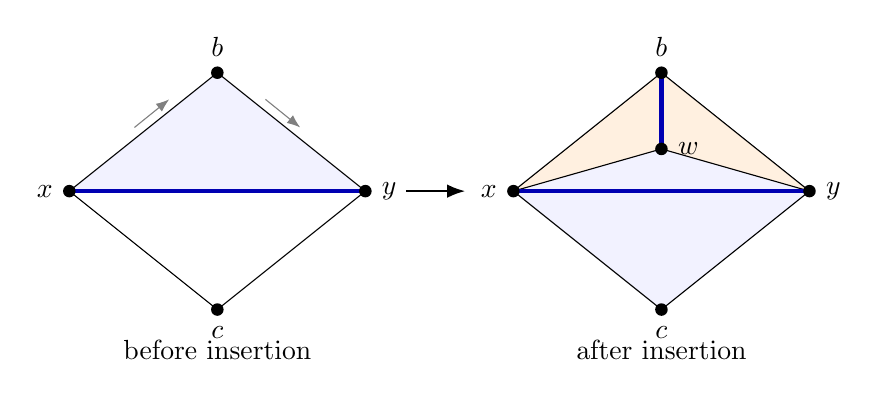
\begin{tikzpicture}[scale=.94,>=Latex,
  v/.style={circle,fill=black,inner sep=1.6pt},
  match/.style={line width=1.5pt,blue!70!black}]
\begin{scope}
\coordinate (x) at (-2,0); \coordinate (y) at (2,0);
\coordinate (b) at (0,1.6); \coordinate (c) at (0,-1.6);
\fill[blue!5] (x)--(b)--(y)--cycle;
\draw (x)--(b)--(y)--(c)--cycle;
\draw[match] (x)--(y);
\draw[->,gray] (-1.12,.86)--(-.65,1.24);
\draw[->,gray] (.65,1.24)--(1.12,.86);
\foreach \p/\pos in {x/left,y/right,b/above,c/below}
 \node[v,label=\pos:$\p$] at (\p) {};
\node at (0,-2.15) {before insertion};
\end{scope}
\draw[->,thick] (2.55,0)--(3.35,0);
\begin{scope}[xshift=6cm]
\coordinate (x) at (-2,0); \coordinate (y) at (2,0);
\coordinate (b) at (0,1.6); \coordinate (c) at (0,-1.6);
\coordinate (w) at (0,.57);
\fill[blue!5] (x)--(w)--(y)--(c)--cycle;
\fill[orange!12] (x)--(b)--(y)--(w)--cycle;
\draw (x)--(b)--(y)--(c)--cycle;
\draw (x)--(w)--(y);
\draw[match] (x)--(y) (b)--(w);
\foreach \p/\pos in {x/left,y/right,b/above,c/below}
 \node[v,label=\pos:$\p$] at (\p) {};
\node[v,label=right:$w$] at (w) {};
\node at (0,-2.15) {after insertion};
\end{scope}
\end{tikzpicture}

\caption{One terminal insertion in the oriented white triangulation.
The old pair has cyclic boundary \((x,b,y,c)\). The new vertex is
\(w\); the thick matching edges are \(xy\) and \(bw\).
The retained pair has polynomial order \((x,w,c,y)\);
the new pair has order \((b,y,x,w)\). All old boundary edges remain.
The arrows record the old first-side orientation.}
\label{td:patch-figure}
\end{figure}

The operation is a stellar subdivision of one face followed by the
displayed matching. The new vertex is fresh and has exactly its
three indicated neighbors, so simplicity is preserved. The three
new triangles each belong to exactly one matched pair. A marked
boundary edge remains a boundary edge and is never promoted to a
matching edge; only \(bw\), which contains a fresh vertex, is added.
Consequently the original mark remains valid even when it bounds
the subdivided triangle.

\subsection{Why an even fan preserves the knot pairing}

In the exposed cyclic tuple define the three possible pairings
\[
 I=\{\{0,3\},\{1,2\}\},\quad
 X=\{\{0,2\},\{1,3\}\},\quad
 H=\{\{0,1\},\{2,3\}\}.
\]
An odd two-strand braid has pairing \(X\), regardless of its sign.
Rotating all labels by one preserves \(X\), so a physically turned
odd terminal still has this pairing.

In the product of two \(X\)'s, the first external lower endpoint
\(F_0\) follows \(F_2,G_1,G_3\) to the upper-left endpoint.
The second follows \(F_1,F_3,G_0,G_2\) to the upper-right endpoint.
These are exactly \(I\), and they use every internal joining
segment. There is no closed internal component. The through
pairing \(I\) is an identity on either side of each of \(I,X,H\);
this follows by following the same two joining strips.
Induction proves:

\begin{lemma}[Even terminal stacks]\label{td:parity}
Any even stack of odd turned terminals preserves the four-endpoint
pairing of the old tangle, on either side, and creates no internal
main component. The signs of the terminal powers are arbitrary.
\end{lemma}

This statement concerns strand connectivity. It does not cancel
the corresponding braid operators. Every inserted crossing circle
remains a distinct component of the augmented link and receives
its own filling integer.

\begin{figure}[htbp]
\centering
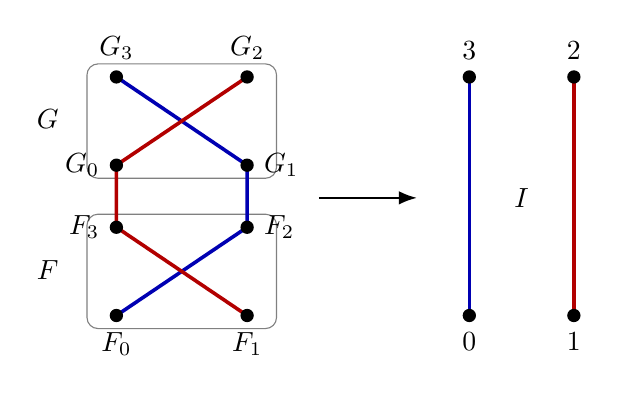
\begin{tikzpicture}[scale=.83,>=Latex,
 p/.style={circle,fill=black,inner sep=1.7pt}]
\draw[rounded corners,gray] (-1.45,-.2) rectangle (1.45,1.55);
\draw[rounded corners,gray] (-1.45,2.1) rectangle (1.45,3.85);
\node at (-2.05,.7) {$F$};
\node at (-2.05,3) {$G$};
\coordinate (f0) at (-1,0); \coordinate (f1) at (1,0);
\coordinate (f2) at (1,1.35); \coordinate (f3) at (-1,1.35);
\coordinate (g0) at (-1,2.3); \coordinate (g1) at (1,2.3);
\coordinate (g2) at (1,3.65); \coordinate (g3) at (-1,3.65);
\draw[blue!70!black,line width=1.3pt] (f0)--(f2)--(g1)--(g3);
\draw[red!70!black,line width=1.3pt] (f1)--(f3)--(g0)--(g2);
\foreach \p/\label/\pos in {f0/F_0/below,f1/F_1/below,f2/F_2/right,
 f3/F_3/left,g0/G_0/left,g1/G_1/right,g2/G_2/above,g3/G_3/above}
 \node[p,label=\pos:$\label$] at (\p) {};
\draw[->,thick] (2.1,1.8)--(3.6,1.8);
\begin{scope}[xshift=5.2cm]
\draw[blue!70!black,line width=1.3pt] (-.8,0)--(-.8,3.65);
\draw[red!70!black,line width=1.3pt] (.8,0)--(.8,3.65);
\foreach \x/\y/\label/\pos in {-.8/0/0/below,.8/0/1/below,
 .8/3.65/2/above,-.8/3.65/3/above}
 \node[p,label=\pos:$\label$] at (\x,\y) {};
\node at (0,1.8) {$I$};
\end{scope}
\end{tikzpicture}

\caption{Endpoint paths through two odd turned terminals. The lower
factor \(F\) is joined to the upper factor \(G\) by
\(F_2G_1\) and \(F_3G_0\). The blue and red paths connect the
external pairs \(0\!-\!3\) and \(1\!-\!2\); every internal endpoint
lies on one path. The crossings in the drawing represent the
pairing \(X\), without fixing the signs of the physical odd powers.}
\label{td:pairing-figure}
\end{figure}

\section{A packing extension which fixes every old circle}

\begin{lemma}[The local interstice]\label{td:interstice}
Let the subdivided triangle have curvatures \(x,b,y\), with
\(x+y>0\). There is a unique disk in its chosen interstice tangent
to those three boundary disks. Its curvature is
\begin{equation}\label{td:one-step}
 b_1=x+y+b+2\sqrt{xb+xy+by}
       =A+b+2\sqrt{Ab+P}.
\end{equation}
Inserting this disk and replacing the shaded faces gives the
complete packing of the subdivided matched sphere, with all
previous circles fixed. The assertion includes marked lines.
\end{lemma}

\begin{proof}
First suppose the three boundary curvatures are positive. Write
\(p_i\) for their centers and \(r_i\) for their radii
\(1/x,1/b,1/y\). Subtract the three squared tangency equations
\(|z-p_i|^2=(r+r_i)^2\), where \(r=1/k\) is the new radius.
Eliminating the two center coordinates gives
\[
 (k-x-b-y)^2=4(xb+xy+by).
 \]
The disk in the bounded interstice takes the plus sign at equal
boundary radii. The two roots never meet for a positive triple,
and the bounded gap and its tangent disk vary continuously with
the boundary radii. Thus this branch is \eqref{td:one-step}
throughout the positive octant.

Here is also a direct model for the labeled supporting faces, which
avoids relying on the tangency equation alone. Apply an
orientation-preserving Möbius map sending one of the three old
contacts to infinity. Rescale so the boundary disks are
\[
 \Im z\le0,\qquad \Im z\ge2,\qquad |z-\ii|\le1 .
 \]
Choose their right-hand interstice. The old shaded outward disk is
\(\Re z>0\), and the new white disk is
\(|z-(2+\ii)|<1\). Its new contacts are \(2,2+2\ii,1+\ii\).
The replacement shaded outward disks are
\begin{equation}\label{td:shaded}
 |z-1|<1,\qquad |z-(1+2\ii)|<1,\qquad \Re z>2 .
\end{equation}
The six old and new contacts form a regular ideal right-angled
octahedron. Its three incident white planes agree with the old
planes, so the corresponding seams are flat.

To check remote supporting inequalities, use the embedded center
triangles supplied by the packing proposition. A bounded shaded
contact disk lies inside its center triangle. A nonincident white
disk meets that triangle, if at all, through its own incident
sectors, whose interiors belong to different center triangles;
it therefore misses the shaded disk. Distinct bounded shaded disks
also have disjoint interiors. For the omitted outer triangle, all
other contacts and bounded disks lie on the inner side of its
contact circle and miss its chosen outward disk.
These statements persist under the normalization above.

The new white disk and all three shaded disks in
\eqref{td:shaded} lie in the old interstice side. They miss every
nonincident old outward disk. Conversely old contacts outside the
attaching face satisfy the new supporting inequalities. The old
and new faces form a closed labeled sphere of exposed supporting
facets. The union of the old polyhedron and the octahedron along
the attaching triangle is therefore their inward halfspace
intersection, with no unintended face or contact. Repeating in
the other projection copy realizes precisely
Lemma~\ref{td:patch}.

Returning to the original marked coordinate leaves every old
circle fixed. One zero curvature is obtained by letting one of
the original circles become a line; the tangency formula has the
continuous value \eqref{td:one-step}. With two zero curvatures the
two marked lines are parallel, and the displayed model applies
directly: the next disk has the same curvature as the old disk.
The case \(x=y=0\) is excluded by \eqref{td:outer}; hence the new
curvature is always positive. Every insertion thus extends the
complete labeled packing on the original marked sphere.
\end{proof}

\begin{figure}[htbp]
\centering
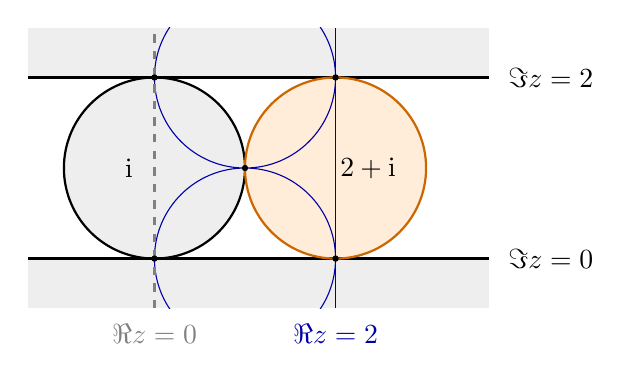
\begin{tikzpicture}[scale=1.15]
\begin{scope}
\clip (-1.4,-.55) rectangle (3.7,2.55);
\fill[gray!13] (-1.4,-.55) rectangle (3.7,0);
\fill[gray!13] (-1.4,2) rectangle (3.7,2.55);
\fill[gray!13] (0,1) circle (1);
\fill[orange!15] (2,1) circle (1);
\draw[black,thick] (-1.4,0)--(3.7,0) (-1.4,2)--(3.7,2);
\draw[black,thick] (0,1) circle (1);
\draw[orange!80!black,thick] (2,1) circle (1);
\draw[blue!65!black] (1,0) circle (1) (1,2) circle (1);
\draw[blue!65!black] (2,-.55)--(2,2.55);
\draw[dashed,gray,thick] (0,-.55)--(0,2.55);
\foreach \x/\y in {0/0,0/2,1/1,2/0,2/2}
 \fill[black] (\x,\y) circle (.035);
\end{scope}
\node at (-.28,1) {$\ii$};
\node at (2.36,1) {$2+\ii$};
\node[anchor=west] at (3.8,2) {$\Im z=2$};
\node[anchor=west] at (3.8,0) {$\Im z=0$};
\node[gray,anchor=north] at (0,-.62) {$\Re z=0$};
\node[blue!65!black,anchor=north] at (2,-.62) {$\Re z=2$};
\end{tikzpicture}

\caption{The normalized interstice. The black lines are
\(\Im z=0,2\); the old and new white disks have centers \(\ii\)
and \(2+\ii\) and radius one. The dashed old shaded boundary is
\(\Re z=0\). The blue circles, centered at \(1,1+2\ii\), and
the blue line \(\Re z=2\) bound the three new outward shaded
disks. The new disk and those shaded disks are contained in the
old right-hand interstice side.}
\label{td:interstice-figure}
\end{figure}

The local normalization is used only to verify the face attachment;
it is not a new choice of marked radius vector in the source.
In the global marked coordinate the protected lines and every
old finite circle remain unchanged. The contact model also shows
that one insertion increases the complete augmented volume by
\(2v_{\rm oct}\), one regular ideal octahedron in each copy.
The volume limit below does not require that numerical increment.

\section{The exact fan recurrence and its finite counts}

Repeat insertion on one side of a retained original region, always
subdividing its current shaded triangle. Let \(b_0=b\). The outer
curvatures \(x,y\), and hence \(A,P\), remain fixed. Put
\(t_j=\sqrt{Ab_j+P}\), taking the nonnegative root. By
\eqref{td:one-step},
\[
 Ab_{j+1}+P=Ab_j+P+A^2+2At_j=(t_j+A)^2.
 \]
Since \(A>0\), this proves the exact solution
\begin{equation}\label{td:recurrence}
 t_j=t_0+jA,\qquad
 b_j=b+2j\sqrt{Ab+P}+j^2A.
\end{equation}
There is no approximation in this recurrence, even when \(b=0\).
Normalize
\[
 u=\sqrt{b/A+\rho},\qquad v=\sqrt{c/A+\rho}.
\]
After \(j,k\) steps on the two sides, respectively,
\begin{equation}\label{td:normalized}
 b_j=A((u+j)^2-\rho),\qquad
 c_k=A((v+k)^2-\rho).
\end{equation}

Choose an integer \(m\) nearest \((v-u)/2\), with either choice
at a tie, and set
\begin{equation}\label{td:counts}
 \begin{aligned}
 L&=\max\left\{0,-m,
       \left\lceil\frac{4-v}{2}\right\rceil,
       \left\lceil\frac{4-u}{2}-m\right\rceil\right\},\\
 j&=2(L+m),\qquad k=2L .
 \end{aligned}
\end{equation}
Both counts are even nonnegative integers and are finite functions
of the original curvatures. They satisfy
\begin{equation}\label{td:balanced-root}
 U=u+j\ge4,\qquad V=v+k\ge4,\qquad |U-V|\le1.
\end{equation}
Indeed the nearest-integer choice gives the last inequality, and
the four entries in the maximum give the other conditions.
Adding the same nonnegative even number to \(j,k\) preserves all
three inequalities. This is a finite construction at each region,
not an eventual assertion without specified counts.

After each insertion the new crossing region consists of the other
two new triangles; neither is subdivided by the next step on the
retained region. Hence previously added regions are not changed
again. Operations at different original regions occur in different
original triangles and preserve their common boundary circles.
Their counts can therefore be chosen from the original packing
independently, and the finite operations can be performed in any
order respecting each side's sequence.

\section{The normalized action and strict balance}

\subsection{A useful elementary comparison}

From the definition of \(e\),
\[
 e(0)=e(1/2)=0,\qquad e'(a)=\log\cot(\pi a),\qquad
 e''(a)=-\frac{2\pi}{\sin(2\pi a)}.
\]
In particular \(e\) is strictly concave and positive in the
interior. The function
\(h(a)=e(a)+a\log(2a)\), extended continuously at zero,
vanishes at both endpoints and has
\[
 h''(a)=-\frac{2\pi}{\sin(2\pi a)}+\frac1a<0.
 \]
Thus \(e(a)>-a\log(2a)\) for \(0<a<1/2\).
Choosing \(a_i=w_i/(2W)\), \(W=\sum_iw_i\), in
\eqref{td:entropy} gives
\begin{equation}\label{td:log-sum}
 \calQ(w_1,w_2,w_3)\ge\tfrac12\log W,
\end{equation}
strictly if at least two weights are positive. This elementary
inequality will settle every newly inserted region.

\subsection{An integral which fixes the retained-region comparison}

The coarser bound \eqref{td:log-sum} alone does not settle the
retained region. Its two new middles are large, and their precise
relative size matters.

For fixed \(x,y\) with \(A>0\) and \(b>0\), the maximizing middle
load is
\begin{equation}\label{td:derivative}
 \frac{\partial}{\partial\log b}\calQ(x,b,y)
       =\frac1\pi\arctan\frac{b}{\sqrt{Ab+P}} .
\end{equation}
For two positive entries the tangent ratios are reciprocal.
For three entries their sum is \(\pi/2\), since
\((Ab+P)=(xb+xy+by)\). The Lagrange multiplier equations
\(e'(a_i)+\log w_i=\text{constant}\) therefore give
\eqref{td:derivative}, as also recorded in
\cite[Lemma 4.1]{Planar}.

Homogeneity gives
\(\calQ(x,b,y)-\frac12\log b=\calQ(x/b,1,y/b)\to0\)
as \(b\to\infty\). To verify the upper limit, a maximizing
sequence cannot keep positive load on a disappearing outer weight:
its negative logarithm would exceed the bounded continuous
entropy. The outer loads therefore tend to zero, and their
entropy tends to zero. The vertex allocation at the middle gives
the reverse bound. Integrating \eqref{td:derivative} from infinity
now proves the absolutely normalized identity
\begin{equation}\label{td:integral}
 \begin{aligned}
 \calQ(x,b,y)&=\tfrac12\log b+R(b),\\
 R(b)&=\frac1\pi\int_b^\infty
          \arctan\frac{\sqrt{At+P}}{t}\,\frac{dt}{t}>0 .
 \end{aligned}
\end{equation}
The integrand is \(O(t^{-3/2})\); the formula also holds when
one outer weight vanishes.

Monotonicity of arctangent, \(P\ge0\), and
\(\arctan z\ge z-z^3/3\) for \(z\ge0\) give
\begin{equation}\label{td:remainder-bound}
 R(b)\ge \frac2\pi\sqrt{\frac Ab}
                 -\frac2{9\pi}\left(\frac Ab\right)^{3/2}.
\end{equation}
The arctangent inequality follows by differentiating the difference;
its derivative is \(z^4/(1+z^2)\ge0\).

\begin{proposition}[The retained region]\label{td:retained}
If \(U,V\) satisfy \eqref{td:balanced-root} and
\[
 b'=A(U^2-\rho),\qquad c'=A(V^2-\rho),
\]
then
\begin{equation}\label{td:margin}
 \calQ(x,b',y)+\calQ(x,c',y)-\max(\log b',\log c')
          >\frac{3347}{27720\min(U,V)}>0.
\end{equation}
\end{proposition}

\begin{proof}
Exchange \(U,V\) if necessary so \(U\ge V\). The quantities
\((U^2-\rho)^{-1/2}\) and \((V^2-\rho)^{-1/2}\) are at most
\(2/\sqrt{63}<\sqrt3\), where \(2w-2w^3/9\) is increasing.
Apply \eqref{td:remainder-bound} and use \(\rho\ge0\) to obtain
\[
 R(b')+R(c')\ge
 \frac2\pi\left(\frac1U+\frac1V\right)
       -\frac2{9\pi}\left(\frac1{U^3}+\frac1{V^3}\right)
 \ge\frac{643}{180\pi V}.
\]
For the last step, \(U\le V+1\le5V/4\), \(U\ge V\) and
\(V^{-3}\le(16V)^{-1}\) give
\(18/5-1/36=643/180\).
The possible mismatch of the two middles satisfies
\[
 \tfrac12\log(b'/c')=
 \int_V^U\frac{t}{t^2-\rho}\,dt
 \le\frac{1}{V(1-1/64)}=\frac{64}{63V}.
\]
Finally \(\pi<22/7\) gives
\[
 \frac{643}{180\pi}-\frac{64}{63}>
 \frac{643\cdot7}{180\cdot22}-\frac{64}{63}
      =\frac{3347}{27720}.
\]
One elementary verification of the strict rational bound is
\(\frac{22}{7}-\pi=\int_0^1 t^4(1-t)^4/(1+t^2)\,dt>0\).
Subtract the logarithmic mismatch from the two positive remainders
in \eqref{td:integral}. This proves \eqref{td:margin}.
\end{proof}

\begin{proposition}[Every added region]\label{td:added}
Every newly inserted region is strictly balanced when it is
created, including all protected-zero cases.
\end{proposition}

\begin{proof}
Its outer pair is \((b,b_1)\), and its middle pair is \((y,x)\)
in the actual argument order. Put \(A'=b+b_1\). Equation
\eqref{td:one-step} gives \(A'\ge x+y=A>0\).
By \eqref{td:log-sum},
\[
 \calQ(b,x,b_1)+\calQ(b,y,b_1)
       \ge\tfrac12\log((A'+x)(A'+y)).
\]
Let \(m=\max(x,y)>0\). Since \(A'\ge m\), the product on the
right is at least \(2m^2\). The sum is consequently larger
than \(\log m\), and hence larger than the logarithm of every
positive middle. A zero middle has no corresponding one-sided
sector. The proof permits \(b=0\); \(b_1>0\) and \(A>0\)
still hold.
\end{proof}

\begin{proof}[Proof of Theorem~\ref{td:main}]
For every original region choose \(j,k\) by \eqref{td:counts}
and perform the two finite sequences. Lemmas~\ref{td:patch}
and \ref{td:interstice} preserve the simple matched sphere,
its mark and every old circle at each step. Formula
\eqref{td:recurrence} computes its retained middle curvatures
exactly. Proposition~\ref{td:retained} gives strict balance
at that region after its two sequences. Proposition~\ref{td:added}
settles every added region, which no later step changes.
Different original regions keep their common old curvatures,
so the argument applies to all of them on one marked packing.
The total number of steps is a finite sum of the explicit counts.
Finally Lemma~\ref{td:parity} gives the endpoint and component
assertions because both counts at every region are even.
\end{proof}

\section{The actual refined source and the filled limit}

The sphere changes, so its invariant also changes. It is important
to identify the new source rather than substitute a scalar
multiplication rule for terminal tangles. Lemma~\ref{td:patch}
fixes the exact two new argument orders in
\eqref{td:local-factors}. Every other local frame is untouched.
One new vertex and one new matched pair are introduced. In
\eqref{td:source}, every original ordinary face keeps its target
\(d=N-1\); the new ordinary face receives one target \(d\).
No additional coefficient is taken at the protected faces.

These statements can also be seen directly in the local winding
data of the exact diagram theorem. Let \(M_f\) count middle
incidences and \(T_f\) count outside minus inside Morse turns,
temporarily restoring the cap at the mark. The local change is
\[
 \Delta M_b=-1,\quad \Delta M_x=\Delta M_y=1,\quad M_w=1,
 \qquad \Delta M_c=0.
\]
For a bounded face, \(M_f-T_f=2\); for the exterior face the
right side is \(-2\). Therefore
\[
 \Delta T_b=-1,\quad \Delta T_x=\Delta T_y=1,\quad T_w=-1,
 \qquad \Delta T_c=0.
\]
The old target exponents are unchanged, and the new exponent
\(\frac d2(T_w-M_w)=-d\) supplies exactly the new target.
At even \(N\), the face parity changes by one across a strand edge
and by zero across a matching edge. Because \(xy\) is matching,
\(\tau_x=\tau_y\), and the unique new clock is
\(\tau_w=\tau_b=\tau_x+1\) modulo two. Thus the new matching
edge \(bw\) and all the new strand edges have the prescribed
parities. These computations agree with the full source theorem,
including its unchanged reduced mark. The extra coupon factor
\(N^{-1}\) is canceled by the new primitive \(N\)-point face grid;
there is no residual quantum-dimension factor.

\begin{lemma}[A certificate at the complete weights]\label{td:certificate}
For a fixed strictly balanced marked sphere, its complete packing
itself is an unabridged shared-weight certificate.
\end{lemma}
\begin{proof}
For an allowed left label with positive overloaded middle \(c\),
\[
 X-A_{\Lft}=
 \min\{X-\log c,\ \calQ(x,c,y)-\tfrac12\log c\}>0.
\]
The first entry is strict balance. The second is the positive
remainder in \eqref{td:integral}, since \(x+y>0\).
The right label is identical with \(b,c\) exchanged. There are
finitely many allowed sides. If there are any, let \(\gamma\)
be the minimum of their positive losses. At the complete vector,
the all-central shared action is \(\Phi_D\). A noncentral string
subtracts at least one loss and no negative loss, so its full
shared rate is at most \(\Phi_D-\gamma\).
This includes globally vanishing strings as well. If no one-sided
label is allowed the certificate is vacuous.
\end{proof}

\begin{proof}[Proof of Corollary~\ref{td:volume}]
Theorem~\ref{td:main} produces a fixed marked simple sphere, and
Lemma~\ref{td:certificate} gives its unabridged certificate.
Apply \cite[Theorem 1.1]{Planar} through
Proposition~\ref{td:imports}. Every original and added crossing
circle retains its own primitive disk slope. Choose
\(\epsilon_e=\pm1\) at added circles, so \eqref{td:powers}
is odd for every integer filling coefficient. The old parity
pattern and Lemma~\ref{td:parity} make the final main component
a knot for every such choice.

The full complementary source has a fixed strict exponential
gap. The Hermite norm costs only the constant
\(\prod_e(1+|n_e|/2)\) for this fixed filling vector. The nonzero
central action tends to the complete action as all \(|n_e|\)
grow independently. Enlarge the threshold so its rate exceeds
the complementary upper rate and so the primitive geometric
completion theorem applies. The full invariant then has the
same rate as that nonzero contribution. The original framing
factor has modulus one, and the primitive action-volume
identity gives \eqref{td:volume-limit}.
Taking \(|p_e|\) sufficiently large implies the required
\(|n_e|\) bound uniformly in the finitely many retained
\(\epsilon_e\)'s. No restriction on ratios of the powers is used.
\end{proof}

There is a combinatorial supply of core knot patterns if none is
specified initially. Form the graph whose vertices are the
untwisted main components and whose edges are the crossing
regions. It is connected because the original contracted
four-valent graph is connected. Choose a spanning tree and switch
exactly those boxes to odd pairing. After any subset of these
switches, the current components are the components of that
forest. The next tree edge joins two different components and
merges them. Induction gives one knot. The signs of these odd
powers are arbitrary, and all subsequent full twists preserve
the pairing. Thus the theorem can start from the finite sphere
and matching, with the parity pattern chosen explicitly.

\section{Exact finite reproduction}

The uniform proofs are the recurrence, the integral inequalities,
the local cut and the finite induction above. The companion
checker provides a second way to catch errors in their finite
formulas:
\begin{verbatim}
python3 papers/terminal-decorations/check.py --output /tmp/terminal-check
\end{verbatim}
It uses the standard Python library and the existing exact
terminal-fan verifier. Polynomial identities are compared in the
ring with relation \(t^2=Ab+P\). The rational constant
\(3347/27720\) is checked exactly. Oriented face cycles are
used to recover the new quartet, and connected components of
the literal pairing graph test both terminal products.
The runner also checks the matching, the protected edge and
the even-level parity extension through sixteen recorded
insertions. Its forty-nine rational count examples are checks
of the formula \eqref{td:counts}; the all-real proof is the
nearest-integer argument above.

The output records source hashes and the exact scope of these
checks. It does not evaluate a knot invariant or replace the
all-length packing, analytic asymptotic or metric-completion
proofs. The new estimates in this paper require no numerical
packing optimizer or sampled saddle point.

\begin{thebibliography}{10}
\bibitem{Finite}
\emph{Finite spectral evaluation and uniform filling bounds}.
\url{https://sashakolpakov.github.io/murakamis_dream/papers/filling-bounds.pdf}.
\bibitem{Local}
\emph{Uniform spectral bounds for local Casimir sources}.
\url{https://sashakolpakov.github.io/murakamis_dream/papers/local-coefficients.pdf}.
\bibitem{Source}
\emph{Holomorphic asymptotics of central shared face coefficients}.
\url{https://sashakolpakov.github.io/murakamis_dream/papers/source-asymptotics.pdf}.
\bibitem{Oscillatory}
\emph{Oscillatory filling sums with independently long twists}.
\url{https://sashakolpakov.github.io/murakamis_dream/papers/oscillatory-fillings.pdf}.
\bibitem{Marked}
\emph{Circle patterns and primitive fillings of augmented links}.
\url{https://sashakolpakov.github.io/murakamis_dream/papers/marked-fillings.pdf}.
\bibitem{Planar}
\emph{Shared face estimates and triangular gluing for planar link diagrams}.
\url{https://sashakolpakov.github.io/murakamis_dream/papers/planar-certificates.pdf}.
\bibitem{Purcell}
J.~S. Purcell, An introduction to fully augmented links,
\emph{Contemp. Math.} \textbf{541} (2011), 205--220.
\url{https://users.monash.edu/~jpurcell/papers/expos-auglinks.pdf}.
\bibitem{Belted}
P. Morgan, B. Ransom, D. Spyropoulos, R. Trapp and C. Ziegler,
Belted sum decompositions of fully augmented links,
\emph{New York J. Math.} \textbf{31} (2025), 1--42.
\url{https://nyjm.albany.edu/j/2025/31-1p.pdf}.
\bibitem{Whitehead}
R. van der Veen, Proof of the volume conjecture for Whitehead chains,
\emph{Acta Math. Vietnam.} \textbf{33} (2008), 421--431.
\url{https://arxiv.org/abs/math/0611181}.
\bibitem{Trivalent}
R. van der Veen, The volume conjecture for augmented knotted
trivalent graphs, \emph{Algebr. Geom. Topol.} \textbf{9} (2009),
691--722.
\url{https://arxiv.org/abs/0805.0094}.
\end{thebibliography}
\end{document}
